%set the master document for easy compilation
%!TEX root = ../D3_5_3.tex

\section{F2.5: ManageLevelAndMode}\label{s:F2.5}

\subsection{Component Requirements}

\begin{longtable}{p{.25\textwidth}p{.7\textwidth}}
\toprule
Component name			& ManageLevelAndMode \\
\midrule
Link to SCADE model		& {\footnotesize \url{https://github.com/openETCS/modeling/tree/master/model/Scade/System/ObuFunctions/ManageLevelsAndModes}} \\
\midrule
SCADE designer			& Marielle Petit-Doche and  Matthias G\"udemann, Systerel \\
\midrule
Description				& Modes and levels define the status of the ETCS
regarding on-board functional status and track infrastructure. \\
\midrule
Input documents	& 
Subset-026, Chapter 4 \newline
Subset-026, Chapter 5 \\
\midrule
Safety integrity level	& 4 \\
\midrule
Time constraints		&  n/a \\
\midrule
API requirements 		&  n/a \\
\bottomrule
\end{longtable}


\subsection{Interface}

An overview of the interface of component ManageLevelAndMode is shown in Figure~\ref{f:mode_and_level} and Figure~\ref{f:mode_and_level_interface}. The inputs and outputs are described in detail in Section~\ref{s:mode_and_level_inputs} respectively \ref{s:mode_and_level_outputs}. Subcomponents are described in Section~\ref{s:mdoe_and_level_subcomponents}.

\begin{figure}
\center
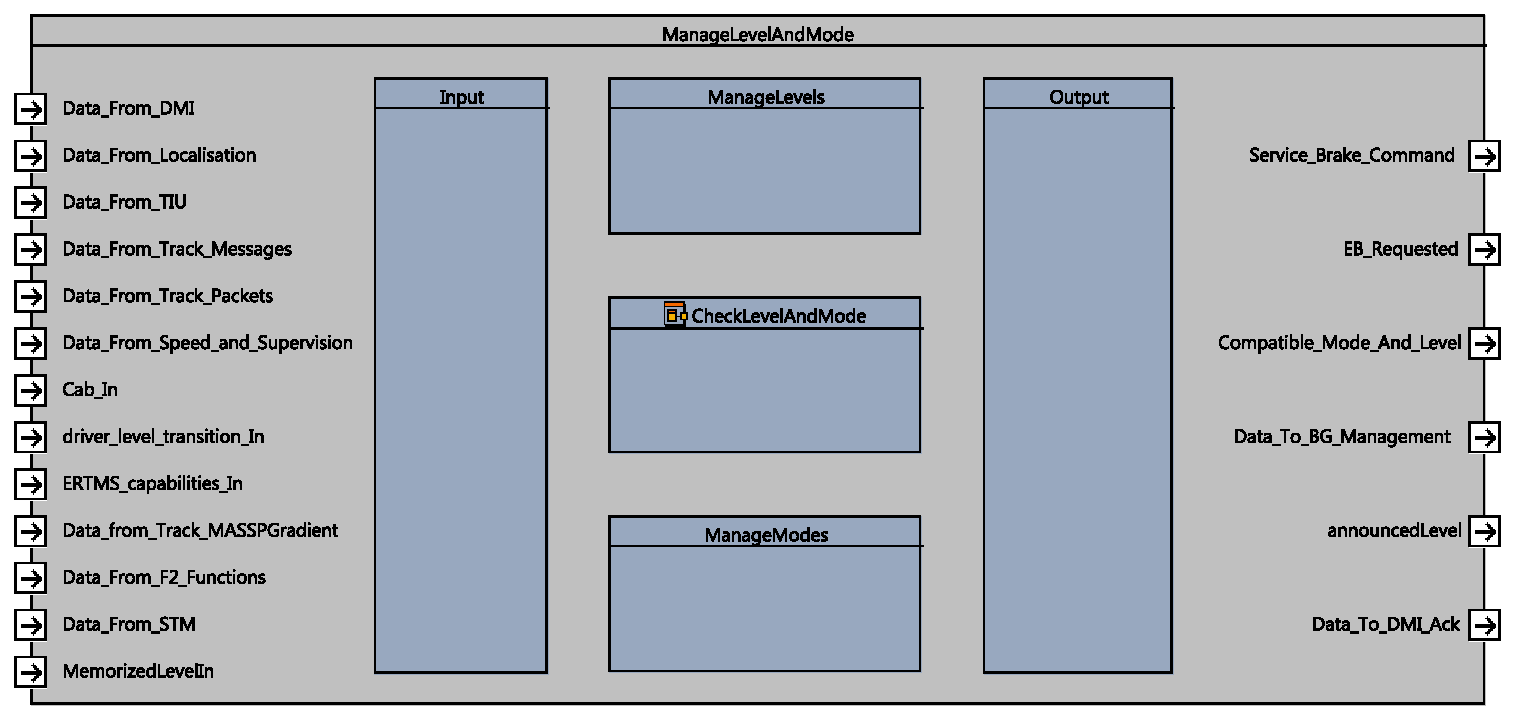
\includegraphics[width=\textwidth]{images/F2_5_ManageLevelsAndModes.pdf}
\caption{ManageLevelAndMode component SysML diagram.}\label{f:mode_and_level}
\end{figure}

\begin{figure}[p]
\center
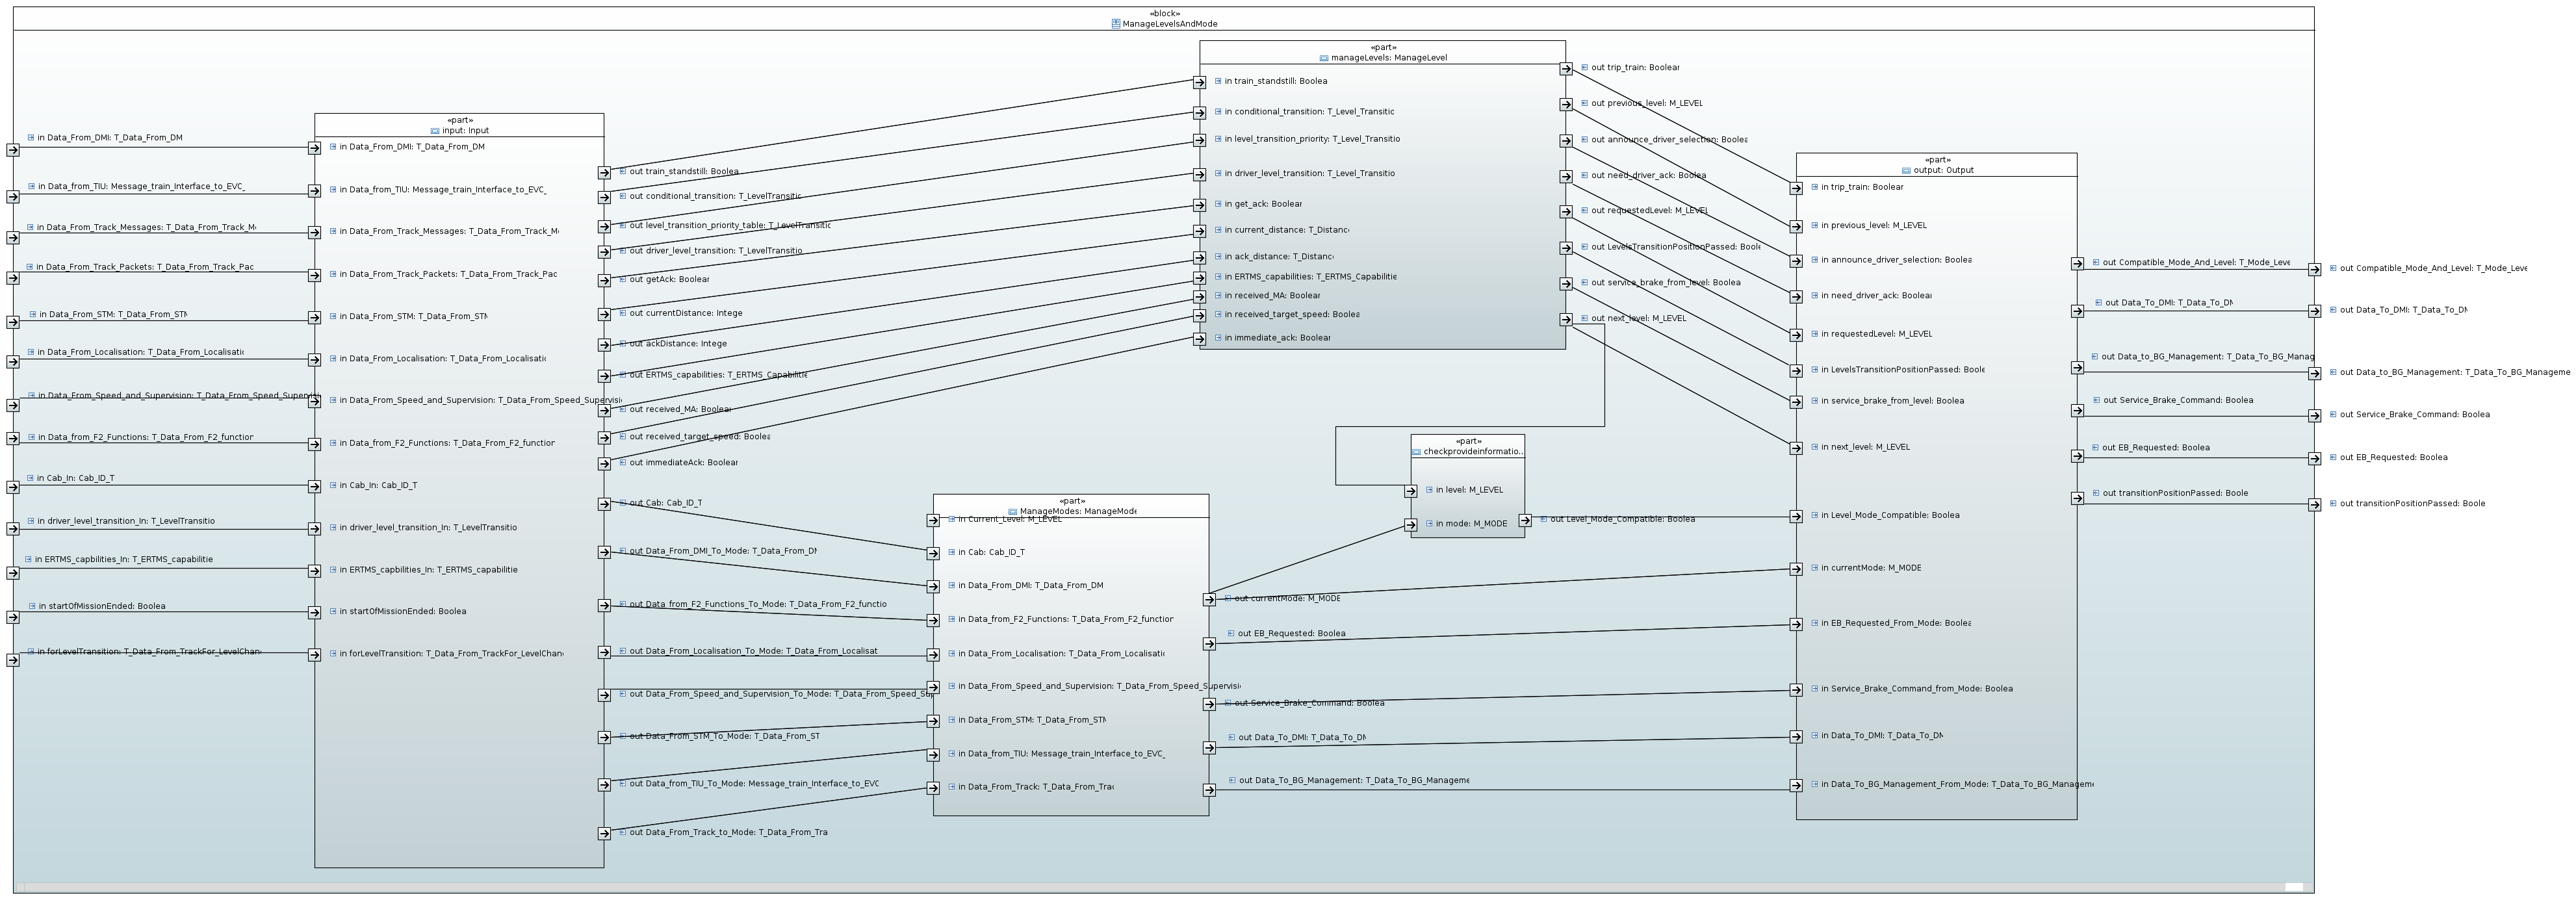
\includegraphics[height=\textheight]{images/ManageLevelsAndModes.png}
\caption{Mode\_and\_Level data flow SysML diagram}\label{f:mode_and_level_interface}
\end{figure}

For a detail description of the interface and contents of the Scade model see \url{https://github.com/openETCS/modeling/blob/master/model/Scade/System/ObuFunctions/ManageLevelsAndModes/ModesAndLevels/ModesAndLevels.pdf}, for types definition see : \url{https://github.com/openETCS/modeling/blob/master/model/Scade/System/ObuFunctions/ManageLevelsAndModes/Level_And_Mode_Types/Level_And_Mode_Types.pdf}

\subsubsection{Inputs}\label{s:mode_and_level_inputs}

See Figure~\ref{f:mode_and_level_inputs} for the inputs of the function.

\begin{figure}
\center
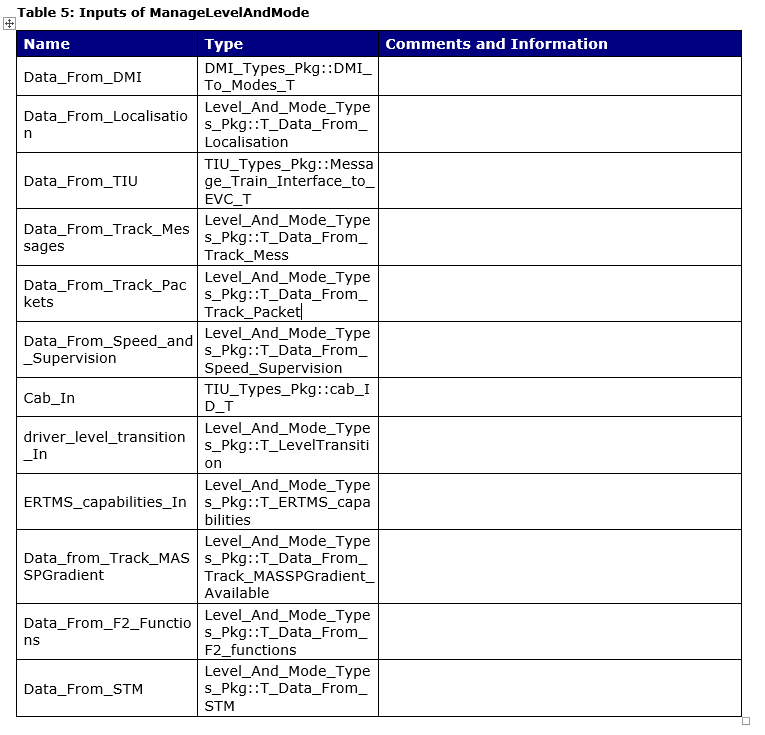
\includegraphics[width=\textwidth]{images/Inputs_ML.png}
\caption{Mode\_and\_Level inputs}\label{f:mode_and_level_inputs}
\end{figure}

\paragraph{Data\_From\_DMI}

\begin{longtable}{p{.25\textwidth}p{.7\textwidth}}
\toprule
Input name				& Data\_From\_DMI \\
\midrule
Description				& Set of data transmitted from DMI  (driver acknowledgements and requests to  switch modes and level) \\
\midrule
Source					& manage\_DMI\_Input\_Pkg::manageDMI\_Input \\ 
\midrule
Type					& DMI\_Types\_Pkg::DMI\_To\_Modes\_T \\
\midrule
Valid range of values	& It is a complex type : \\
& \begin{itemize}
\item valid :  bool,  flag to inform of the freshness of the information
\item DriverAck : DMI\_DriverAck\_T, indicate which mode is acknoledged
\item DriverRequest : DMI\_DriverRequest\_T, table of boolean values for all the driver request related to  mode changes.
\item LevelAck : bool, indication of Level  change acknowledgement
\end{itemize} \\
\midrule
Behaviour when value is at boundary	& n/a \\ 
\midrule
Behaviour for values out of valid range	& n/a \\ 
\midrule
Behaviour when value is erroneous, absent or unwanted (i.e. spurious) & n/a \\ 
\bottomrule
\end{longtable}

\paragraph{Data\_From\_Localisation}

\begin{longtable}{p{.25\textwidth}p{.7\textwidth}}
\toprule
Input name				& Data\_From\_Localisation \\
\midrule
Description				& Set of data on position and speed of the train \\
\midrule
Source					& ???? \todo[inline]{to be completed} \\ 
\midrule
Type					& Level\_And\_Mode\_Types\_Pkg::T\_Data\_From\_Localisation \\
\midrule
Valid range of values	& It is a complex type : \\
& \begin{itemize}
\item BG\_In\_List\_Expected\_BG\_In\_SR : bool,
\item  BG\_In\_List\_Expected\_BG\_In\_SH : bool, 
\item PositionErrors : TrainPosition\_Types\_Pck::positionErrors\_T,
\item  Train\_Position : TrainPosition\_Types\_Pck::trainPosition\_T,
\item Train\_Speed : Obu\_BasicTypes\_Pkg::Speed\_T, 
\item Train\_Standstill : bool
\end{itemize} \\
\midrule
Behaviour when value is at boundary	& n/a \\ 
\midrule
Behaviour for values out of valid range	& n/a \\ 
\midrule
Behaviour when value is erroneous, absent or unwanted (i.e. spurious) & n/a \\ 
\bottomrule
\end{longtable}

\paragraph{Data\_From\_TIU}

\begin{longtable}{p{.25\textwidth}p{.7\textwidth}}
\toprule
Input name				& Data\_From\_TIU \\
\midrule
Description				& Set of data providing by TIU \\
\midrule
Source					& input\_from\_TIU\_API\_Pkg::manageTIU\_input \\ 
\midrule
Type					& TIU\_Types\_Pkg::Message\_Train\_Interface\_to\_EVC\_T \\
\midrule
Valid range of values	& It is a complex type defined in the TIU package \\
\midrule
Behaviour when value is at boundary	& n/a \\ 
\midrule
Behaviour for values out of valid range	& n/a \\ 
\midrule
Behaviour when value is erroneous, absent or unwanted (i.e. spurious) & n/a \\ 
\bottomrule
\end{longtable}


\paragraph{Data\_From\_Track\_Messages}

\begin{longtable}{p{.25\textwidth}p{.7\textwidth}}
\toprule
Input name				& Data\_From\_Track\_Messages \\
\midrule
Description				& Messages received from trackside contaigning information for modes and levels switches \\
\midrule
Source					& ???? 
\todo[inline]{to be completed}\\ 
\midrule
Type					& Level\_And\_Mode\_Types\_Pkg::T\_Data\_From\_Track\_Messages \\
\midrule
Valid range of values	& It is a complex type containing the information of messages : 2, 6, 15, 16, 27 and 28 \\
\midrule
Behaviour when value is at boundary	& n/a \\ 
\midrule
Behaviour for values out of valid range	& n/a \\ 
\midrule
Behaviour when value is erroneous, absent or unwanted (i.e. spurious) & n/a \\ 
\bottomrule
\end{longtable}


\paragraph{Data\_From\_Track\_Packets}

\begin{longtable}{p{.25\textwidth}p{.7\textwidth}}
\toprule
Input name				& Data\_From\_Track\_Packets \\
\midrule
Description				& Packets received from trackside contaigning information for modes and levels switches \\
\midrule
Source					& ???? 
\todo[inline]{to be completed}\\ 
\midrule
Type					& Level\_And\_Mode\_Types\_Pkg::T\_Data\_From\_Track\_Packet \\
\midrule
Valid range of values	& It is a complex type containing the information of packets : 12, 15, 21, 27, 41, 46, 63, 80, 135, 137, 138 and 139 \\
\midrule
Behaviour when value is at boundary	& n/a \\ 
\midrule
Behaviour for values out of valid range	& n/a \\ 
\midrule
Behaviour when value is erroneous, absent or unwanted (i.e. spurious) & n/a \\ 
\bottomrule
\end{longtable}




\paragraph{Data\_From\_speed\_and\_Supervision}


\begin{longtable}{p{.25\textwidth}p{.7\textwidth}}
\toprule
Input name				& Data\_From\_speed\_and\_Supervision \\
\midrule
Description				& Data provided by the speed and supervision function \\
\midrule
Source					& Speed and Supervision function
\todo[inline]{Please use exact component name from SCADE model.} \\ 
\midrule
Type					& Level\_And\_Mode\_Types\_Pkg::T\_Data\_From\_Speed\_Supervision \\
\midrule
Valid range of values	& Input type a complex type
\begin{itemize}
\item \emph{Estim\_front\_End\_overpass\_SR\_Dist : bool}: the train overpass the SR distance with its estimated front end (from SR to trip mode condition 42) 
\item \emph{Estim\_Front\_End\_Rear\_SSP : bool}: estimated front end is rear of the start location of either SSP or gradient profile stored on-board (from FS, LS, OS to trip mode condition 69)
\item \emph{Override\_Function\_Active}: boolean to indicate the state of the activation function 	  	
\item \emph{EOA\_Antenna\_Overpass : bool}: the train overpasses the  EOA  with min safe antenna position Level 1 (from FS, LS, OS to trip mode condition 12)
\item \emph{EOA\_Front\_End : bool} the train overpasses the  EOA  with min safe front end, Level 2 or 3 (from FS, LS, OS to trip mode condition 16)
\item \emph{Train\_Speed\_Under\_Overide\_Limit : bool} supervision when override function is active (to SR mode condition 37)
\end{itemize}\\
\midrule
Behaviour when value is at boundary	& n/a \\ 
\midrule
Behaviour for values out of valid range	& n/a \\ 
\midrule
Behaviour when value is erroneous, absent or unwanted (i.e. spurious) & n/a \\ 
\bottomrule
\end{longtable}



\paragraph{driver\_level\_transition\_in}

\begin{longtable}{p{.25\textwidth}p{.7\textwidth}}
\toprule
Input name				& driver\_level\_transition\_in \\
\midrule
Description				& Request of level transition given by the driver for example at start of mission \\
\midrule
Source					& manage\_DMI\_Input\_Pkg::manageDMI\_Input \\ 
\midrule
Type					& Level\_And\_Modes\_Types\_Pkg::T\_LevelTransition \\
\midrule
Valid range of values	& It is a complex type:  \\
& \begin{itemize}
\item is\_set : bool,
\item transition : Level\_And\_Mode\_Types\_Pkg::T\_LevelTansitionInfo, 
\item LRBG : NID\_LRBG, 
\item referenceLocation : Obu\_BasicTypes\_Pkg::L\_internal\_Type
\end{itemize} \\
\midrule
Behaviour when value is at boundary	& n/a \\ 
\midrule
Behaviour for values out of valid range	& n/a \\ 
\midrule
Behaviour when value is erroneous, absent or unwanted (i.e. spurious) & n/a \\ 
\bottomrule \\ 
\end{longtable}


\paragraph{Cab\_In}

\begin{longtable}{p{.25\textwidth}p{.7\textwidth}}
\toprule
Input name				& Cab\_In \\
\midrule
Description				& Identification of the cabine where the EVC is implemented \\
\midrule
Source					& TIU \\ 
\midrule
Type					& TIU\_Types\_Pkg::cab\_ID\_T \\
\midrule
Valid range of values	&  [CabUndefined, CabA, CabB] \\
\midrule
Behaviour when value is at boundary	& n/a \\ 
\midrule
Behaviour for values out of valid range	& n/a \\ 
\midrule
Behaviour when value is erroneous, absent or unwanted (i.e. spurious) & n/a \\ 
\bottomrule
\end{longtable}


\paragraph{ERTMS\_Capabilities}

\begin{longtable}{p{.25\textwidth}p{.7\textwidth}}
\toprule
Input name				& ERTMS\_Capabilities \\
\midrule
Description				& Identification of the capabilities of the train in regards of ERTMS levels\\
\midrule
Source					& ??? 
\todo[inline]{to be completed}\\ 
\midrule
Type					& T\_ERTMS\_Capabilities \\
\midrule
Valid range of values	& It is a complex type:  \\
& \begin{itemize}
\item NTC : bool,
\item L0 : bool, 
\item L1 : bool, 
\item L2 : bool,
\item L3 : bool
\end{itemize} \\
\midrule
Behaviour when value is at boundary	& n/a \\ 
\midrule
Behaviour for values out of valid range	& n/a \\ 
\midrule
Behaviour when value is erroneous, absent or unwanted (i.e. spurious) & n/a \\ 
\bottomrule
\end{longtable}




\paragraph{Data\_From\_Track\_MASSPGradient}

\begin{longtable}{p{.25\textwidth}p{.7\textwidth}}
\toprule
Input name				& Data\_From\_Track\_MASSPGradient \\
\midrule
Description				& Information that some packets have been received from trackside c \\
\midrule
Source					& ???? 
\todo[inline]{to be completed}\\ 
\midrule
Type					& Level\_And\_Mode\_Types\_Pkg::T\_Data\_From\_Track\_MASSPGradient \\
\midrule
Valid range of values	& It is a complex type containing the information of packets : 12, 15, 21, 27 \\
\midrule
Behaviour when value is at boundary	& n/a \\ 
\midrule
Behaviour for values out of valid range	& n/a \\ 
\midrule
Behaviour when value is erroneous, absent or unwanted (i.e. spurious) & n/a \\ 
\bottomrule
\end{longtable}



\paragraph{Data\_From\_F2\_Functions}

\begin{longtable}{p{.25\textwidth}p{.7\textwidth}}
\toprule
Input name				& Data\_From\_F2\_Functions \\
\midrule
Description				& Information received from other F2 functions \\
\midrule
Source					& ???? 
\todo[inline]{to be completed}\\ 
\midrule
Type					& Level\_And\_Mode\_Types\_Pkg::T\_Data\_From\_F2\_Functions \\
\midrule
Valid range of values	& It is a complex type : \\
& \begin{itemize}
\item Common\_Errors : Common\_Types\_Pkg::MSG\_Errors\_T, 
\item Failure\_Occured : bool,, 
\item Continue\_Shunting\_Active : bool, 
\item  Stop\_Shunting\_Stored : bool
\end{itemize} \\
\midrule
Behaviour when value is at boundary	& n/a \\ 
\midrule
Behaviour for values out of valid range	& n/a \\ 
\midrule
Behaviour when value is erroneous, absent or unwanted (i.e. spurious) & n/a \\ 
\bottomrule
\end{longtable}



\paragraph{Data\_From\_STM}

\begin{longtable}{p{.25\textwidth}p{.7\textwidth}}
\toprule
Input name				& Data\_From\_STM \\
\midrule
Description				& Information concerning STM embedded systems \\
\midrule
Source					& ???? 
\todo[inline]{to be completed}\\ 
\midrule
Type					& Level\_And\_Mode\_Types\_Pkg::T\_Data\_From\_STM \\
\midrule
Valid range of values	& It is a complex type : \\
& \begin{itemize}
\item Interface\_to\_National\_System : bool,, 
\item  National\_Trip\_Order : bool
\end{itemize} \\
\midrule
Behaviour when value is at boundary	& n/a \\ 
\midrule
Behaviour for values out of valid range	& n/a \\ 
\midrule
Behaviour when value is erroneous, absent or unwanted (i.e. spurious) & n/a \\ 
\bottomrule
\end{longtable}



\subsubsection{Outputs}\label{s:mode_and_level_outputs}

\begin{figure}
\center
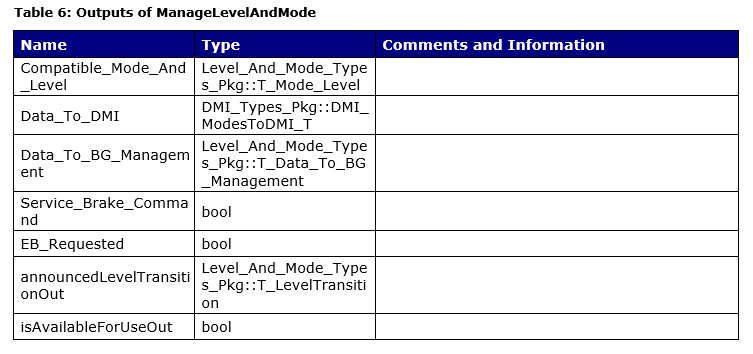
\includegraphics[width=\textwidth]{images/Outputs_ML.png}
\caption{Mode\_and\_Level outputs}\label{f:mode_and_level_outputs}
\end{figure}



\paragraph{Compatible\_Mode\_And\_Level}

\begin{longtable}{p{.25\textwidth}p{.7\textwidth}}
\toprule
Output name				& Compatible\_Mode\_And\_Level \\
\midrule
Description				& Structure containing mode and lavel information  \\
\midrule
Destination				& all the components  \\ 
\midrule
Type					& Level\_And\_Mode\_Types\_Pkg::T\_Mode\_Level \\
\midrule
Valid range of values	& It is a complex type : \\
& \begin{itemize}
\item CompatibleModeAndLevel : bool,
\item level : M\_LEVEL,
\item newLevel : bool,
\item mode : M\_MODE, 
\item newMode : bool
\end{itemize} \\
\midrule
Behaviour when value is at boundary	& n/a \\ 
\midrule
Behaviour for values out of valid range	& n/a \\ 
\midrule
Behaviour when value is erroneous, absent or unwanted (i.e. spurious) & n/a \\
\bottomrule
\end{longtable}

\paragraph{Data\_To\_DMI}

\begin{longtable}{p{.25\textwidth}p{.7\textwidth}}
\toprule
Output name				& Data\_To\_DMI \\
\midrule
Description				& Data information to provide to the driver  \\
\midrule
Destination				& all the components  \\ 
\midrule
Type					& DMI\_Types\_Pkg::DMI\_ModesToDMI\_T \\
\midrule
Valid range of values	& It is a complex type defined in the DMI package \\
\midrule
Behaviour when value is at boundary	& n/a \\ 
\midrule
Behaviour for values out of valid range	& n/a \\ 
\midrule
Behaviour when value is erroneous, absent or unwanted (i.e. spurious) & n/a \\
\bottomrule
\end{longtable}

\paragraph{Data\_To\_BG\_Management}

\begin{longtable}{p{.25\textwidth}p{.7\textwidth}}
\toprule
Output name				& Data\_To\_BG\_Management \\
\midrule
Description				& Set of data concerning BG management \\
\midrule
Destination				& all the components  \\ 
\midrule
Type					& Level\_And\_Mode\_Types\_Pkg::T\_Data\_To\_BG\_Management \\
\midrule
Valid range of values	& It is a complex type : \\
& \begin{itemize}
\item EoM\_Procedure\_req : bool,
\item  Clean\_BG\_List\_SH\_Area : bool, 
\item MA\_Req : bool,
\item  Req\_for\_SH\_from\_Driver : bool,
\item Connection\_to\_RBC\_req : bool, 
\item Position\_Repport\_Needed : bool
\end{itemize} \\
\midrule
Behaviour when value is at boundary	& n/a \\ 
\midrule
Behaviour for values out of valid range	& n/a \\ 
\midrule
Behaviour when value is erroneous, absent or unwanted (i.e. spurious) & n/a \\
\bottomrule
\end{longtable}


\paragraph{Sevice\_Brake\_Command}

\begin{longtable}{p{.25\textwidth}p{.7\textwidth}}
\toprule
Output name				& Sevice\_Brake\_Command \\
\midrule
Description				& Command of the Service brake \\
\midrule
Destination				& all the components \\ 
\midrule
Type					& bool \\
\midrule
Valid range of values	&  \\
\midrule
Behaviour when value is at boundary	& n/a \\ 
\midrule
Behaviour for values out of valid range	& n/a \\ 
\midrule
Behaviour when value is erroneous, absent or unwanted (i.e. spurious) & n/a \\
\bottomrule
\end{longtable}

\paragraph{EB\_Requested}

\begin{longtable}{p{.25\textwidth}p{.7\textwidth}}
\toprule
Output name				& EB\_Requested \\
\midrule
Description				& Command of the Emergency brake \\
\midrule
Destination				& all the components \\ 
\midrule
Type					& bool \\
\midrule
Valid range of values	&  \\
\midrule
Behaviour when value is at boundary	& n/a \\ 
\midrule
Behaviour for values out of valid range	& n/a \\ 
\midrule
Behaviour when value is erroneous, absent or unwanted (i.e. spurious) & n/a \\
\bottomrule
\end{longtable}



\paragraph{announcedLevelTransition}

\begin{longtable}{p{.25\textwidth}p{.7\textwidth}}
\toprule
Input name				& announcedLevelTransition \\
\midrule
Description				& Level transition selected for an immediate or future switch \\
\midrule
Destination				& all the components \\ 
\midrule
Type					& Level\_And\_Modes\_Types\_Pkg::T\_LevelTransition \\
\midrule
Valid range of values	& It is a complex type:  \\
& \begin{itemize}
\item is\_set : bool,
\item transition : Level\_And\_Mode\_Types\_Pkg::T\_LevelTansitionInfo, 
\item LRBG : NID\_LRBG, 
\item referenceLocation : Obu\_BasicTypes\_Pkg::L\_internal\_Type
\end{itemize} \\
\midrule
Behaviour when value is at boundary	& n/a \\ 
\midrule
Behaviour for values out of valid range	& n/a \\ 
\midrule
Behaviour when value is erroneous, absent or unwanted (i.e. spurious) & n/a \\ 
\bottomrule \\ 
\end{longtable}


\paragraph{isAvailableForUse}

\begin{longtable}{p{.25\textwidth}p{.7\textwidth}}
\toprule
Output name				& isAvailableForUse \\
\midrule
Description				& the output announcedLevelTransition is available for use, ie. correspond to ERTMS capabilities of the train \\
\midrule
Destination				& all the components \\ 
\midrule
Type					& bool \\
\midrule
Valid range of values	&  \\
\midrule
Behaviour when value is at boundary	& n/a \\ 
\midrule
Behaviour for values out of valid range	& n/a \\ 
\midrule
Behaviour when value is erroneous, absent or unwanted (i.e. spurious) & n/a \\
\bottomrule
\end{longtable}



\subsection{Subcomponents}\label{s:mdoe_and_level_subcomponents}

\subsubsection{Level\_Management}
%set the master document for easy compilation
%!TEX root = ../D3_5_3.tex

\paragraph{Component Requirements}

\begin{longtable}{p{.25\textwidth}p{.7\textwidth}}
\toprule
Component name			& Level\_Management \\
\midrule
Link to SCADE model		& {\footnotesize \url{https://github.com/openETCS/modeling/tree/master/openETCS ArchitectureAndDesign/Work Groups/Group 3/SCADE/LevelManagement/}} \\
\midrule
SCADE designer			& Marielle Petit-Doche and  Matthias G\"udemann, Systerel \\
\midrule
Description				& The level management subsystem receives level transition order tables and selects the order with the highest probability. It stores the information about the selected transition order and transits to the requested level once the train passes the location of the level transition.

If required, the driver is asked to acknowledge the transition, in case of no acknowledgment or if conditions for the level transition are not fulfilled, the train gets tripped.

On the most abstract level the design consists of the \emph{manage\_priorities} function which takes the level transition order priority tables as inputs and computes the highest priority transition.

This transition order is the fed to the \emph{computeLevelTransitions} operator. This operator consists of three main parts. The \emph{ComputeTransitionConditions} operator that emits the fulfilled conditions to change from a given level to a new level, the \emph{LevelStateMachine} that stores the current level and takes the computed change conditions as input for possible level transitions and finally the \emph{driverAck} operator which contains a state machine that stores the information whether the system is currently waiting for a driver acknowledge and emits the train trip information if necessary. \\
\midrule
Input documents	& 
Subset-026, Chapter 5.10 \\
\midrule
Safety integrity level		& 4 \\
\midrule
Time constraints		& [If applicable description of time constraints, otherwise n/a] 
\todo[inline]{to be completed}\\
\midrule
API requirements 		& [If applicable description of API requirements, otherwise n/a] 
\todo[inline]{to be completed}\\
\bottomrule
\end{longtable}


\paragraph{Interface}

For an overview of the interface of this internal component we refer to the SCADE model (cf.~link above) respectively the SCADE generated documentation.

\subsubsection{Mode\_Management}
%set the master document for easy compilation
%!TEX root = ../D3_5_2.tex

\paragraph{Component Requirements}

\begin{longtable}{p{.25\textwidth}p{.7\textwidth}}
\toprule
Component name			& Mode\_Management \\
\midrule
Link to SCADE model		& {\footnotesize \url{https://github.com/openETCS/modeling/tree/master/model/Scade/System/ObuFunctions/ManageLevelsAndModes/Modes}} \\
\midrule
SCADE designer			& Marielle Petit-Doche, Systerel \\
\midrule
Description				& This function is in charge of the computation of new mode to apply according to conditions from inputs (track information, driver interactions, train data,...) and other functions.

Three subfunctions are defined:
\begin{description}
\item[Inputs] proceeds to inputs check and preparation.
\item[ComputeModesCondition] performs all specific procedure linked to mode management and defined in  \citep{subset-026} sections 5.4, 5.5, 5.6, 5.7, 5.8, 5.9, 5.11, 5.12, 5.13, 5.19 and specifies the conditions to define a mode transition according condition table of section 4.6.3 of \citep{subset-026}
\item[SwitchModes] performs the mode selection according the conditions and priorities defined in transition table  section 4.6.2 of \citep{subset-026}
\item[Outputs] prepares packet of outputs.
\end{description} \\
\midrule
Input documents	& 
Subset-026, Chapter 4.4, 4.6, 5.4, 5.5, 5.6, 5.7, 5.8, 5.9, 5.11, 5.12, 5.13, 5.19 \\
\midrule
Safety integrity level		& 4 \\
\midrule
Time constraints		& [If applicable description of time constraints, otherwise n/a] \\
\midrule
API requirements 		& [If applicable description of API requirements, otherwise n/a] \\
\bottomrule
\end{longtable}


\paragraph{Interface}

For an overview of the interface of this internal component we refer to the SCADE model (c.f.~link above) respectively the SCADE generated documentation.

\subsubsection{Check\_and\_Provide\_Mode\_and\_Level}
%set the master document for easy compilation
%!TEX root = ../D3_5_3.tex

\paragraph{Component Requirements}

\begin{longtable}{p{.25\textwidth}p{.7\textwidth}}
\toprule
Component name			& Check\_and\_Provide\_Mode\_and\_Level \\
\midrule
Link to SCADE model		& {\footnotesize \url{https://github.com/openETCS/modeling/tree/master/model/Scade/System/ObuFunctions/ManageLevelsAndModes/Modes}} \\
\midrule
SCADE designer			& Marielle Petit-Doche, Systerel \\
\midrule
Description				& Checks compatibility between mode and level and provides outputs. \\
\midrule
Input documents	& 
Subset-026, Chapter 3.6.5 \\
\midrule
Safety integrity level		& 4 \\
\midrule
Time constraints		& [If applicable description of time constraints, otherwise n/a] \\
\midrule
API requirements 		& [If applicable description of API requirements, otherwise n/a] \\
\bottomrule
\end{longtable}


\paragraph{Interface}

For an overview of the interface of this internal component we refer to the SCADE model (c.f.~link above) respectively the SCADE generated documentation.


